\documentclass[10pt,a4paper]{article}
\usepackage[utf8]{inputenc}
\usepackage[english]{babel}
\usepackage[T1]{fontenc}
\usepackage{amsmath}
\usepackage{amsfonts}
\usepackage{amssymb}
\usepackage{subcaption}
\usepackage{makeidx}
\usepackage{graphicx}
\usepackage{fourier}
\usepackage{listings}
\usepackage{color}
\usepackage{hyperref}
\usepackage[left=2cm,right=2cm,top=2cm,bottom=2cm]{geometry}
\author{Tommy Müller, Marcus Dittrich, Vincent Noculak}
\title{Rastertunnelmikroskopie}

\lstset{language=C++,
	keywordstyle=\bfseries\color{blue},
	commentstyle=\itshape\color{red},
	stringstyle=\color{green},
	identifierstyle=\bfseries,
	frame=single}
\begin{document}

\maketitle
\newpage
\tableofcontents
\newpage

\section{Versuchsauswertung}

\subsection{Ebene Fläche auf der Grafitoberfläche}

Wir sollten eine Ebene Fläche im Grafit finden und versuchen anhand dieser die Atomare Struktur des Grafits darzustellen. Obwohl wir Ebene Flächen im Grafit fanden, war es nicht möglich Atomare Strukturen zu erkennen. Dies lag wahrscheinlich daran, dass die Spitze unseres Sensors nicht spitz genug war. Deshalb haben wir zur Untersuchung der Atomaren Struktur die Daten aus den Referenzmaterialien genommen. Die Messung aus den Referenzmaterialien kann in \ref{Grafitoberflächenebene} gesehen werden. Hier ist \ref{grafob1} die rohe Messung an sich. In \ref{grafob2} haben wir mithilfe einer doppelten Fouriertransformation Störung aus der Messung entfernt. Dadurch lässt sich sie atomare Struktur genauer erkennen und untersuchen.

\begin{figure}[h]
	\centering
	\begin{subfigure}{0.45\textwidth}
		\centering
		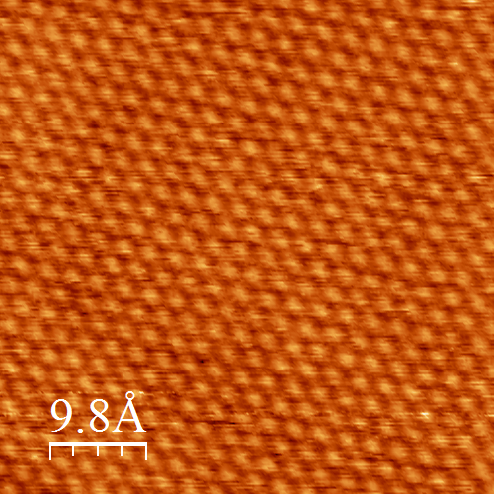
\includegraphics[width=\textwidth]{vor_doppelter_fourier.png}
		\caption{gemessene Grafitoberfläche}
		\label{grafob1}
	\end{subfigure}
	\begin{subfigure}{0.45\textwidth}
		\centering
		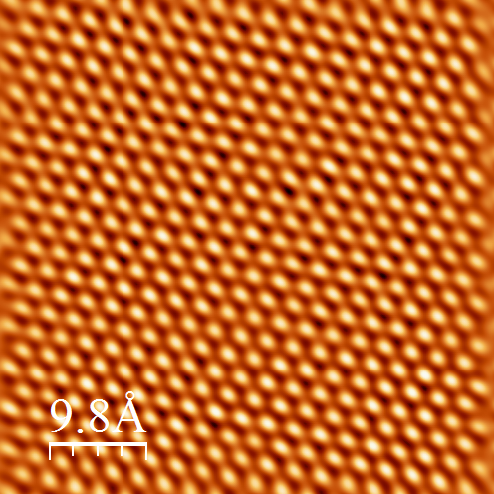
\includegraphics[width=\textwidth]{nach_doppelter_fourier.png}
		\caption{Gemessene Grafitoberfläche, nachdem Störungen durch eine doppelte Fouriertransformation beseitigt wurden}
		\label{grafob2}
	\end{subfigure}

	\caption{Messung des Tunnelstroms an einer ebenen Fläche Grafit}
	\label{Grafitoberflächenebene}
\end{figure}

Es kann klar erkannt werden, dass die Kohlenstoffatome regelmäßig in einer Kristallstruktur angeordnet sind. Man erkennt ein hexagonales Kristallsystem, wie es für Grafit zu erwarten war.

\begin{figure}[h]
	\centering

	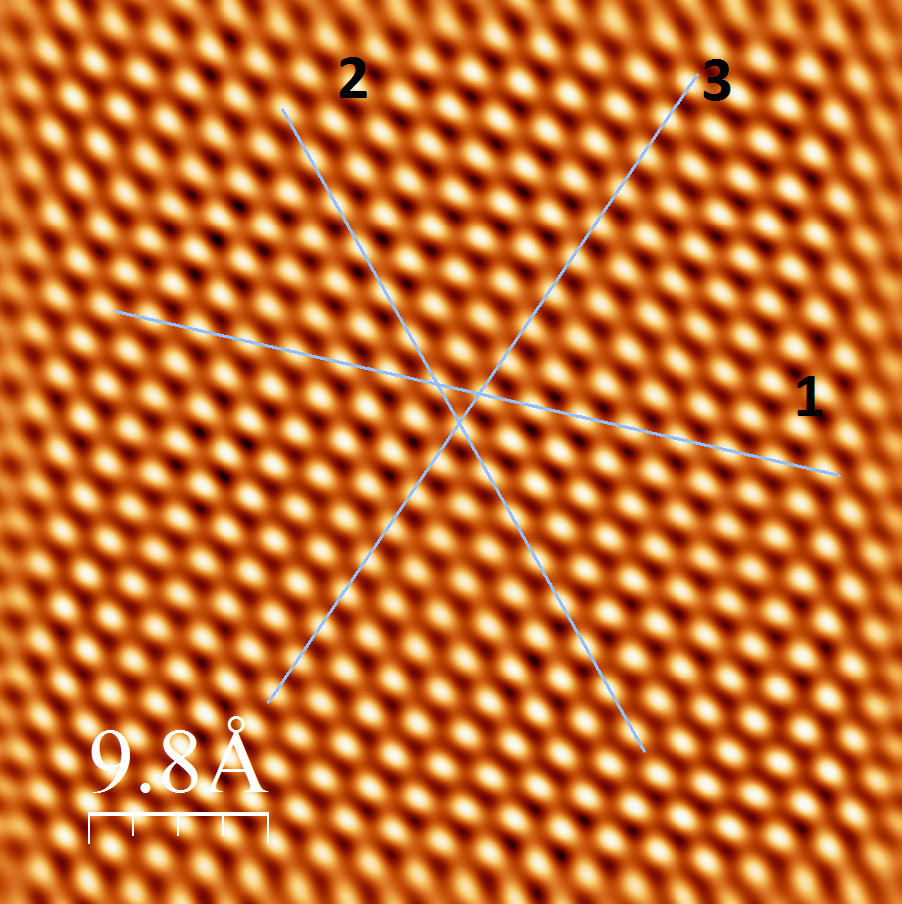
\includegraphics[scale = 0.6]{Aufnahme_Ebene_doppelte_fourier2.png}

	\caption{Messung der Abstände der atomaren Erhebungen}
	\label{Messungerh1}
\end{figure}

Entlang der in \ref{Messungerh1} zu sehenden Linie haben wir die Abstände der Atomaren Erhebungen gemessen. Das dazugehörige Diagramm kann in Abbildung \ref{Messungerh2} gesehen werden. Wir haben alle Abstände entlang der zu sehenden Gerade gemessen und anschließend einen Mittelwert mit Standartabweichung gebildet. Die gemessenen Abstände sind in Tabelle \ref{Messungerh5} zu sehen. Unser Wert für den Abstand der atomaren Erhebungen ist $(0,266 \pm 0,001) nm$.

Laut der Theorie sehen wir in dem mit dem Rastertunnelmikroskop aufgenommenen Bild nur jedes zweite Atom des Grafit-Kristalls. Der planare Abstand nächster Nachbarn im Kristall ist mit $b = 0,142 nm$ gegeben. Der von uns zu erwartende Abstand der atomaren Erhebungen lässt sich dann mithilfe des Kosinussatzes als 

\begin{equation}
	s = b \cdot \sqrt{2(1-cos(120^\circ))} = 0,2460 nm
\end{equation}

berechnen. Auch wenn unserer gemessener Wert bis zur ersten signifikanten Stelle mit diesem theoretischen Wert übereinstimmt, liegt dieser wegen der kleinen Standartabweichung nicht innerhalb des dritten Fehlerintervalls.

\begin{figure}[h]
	\centering
	
	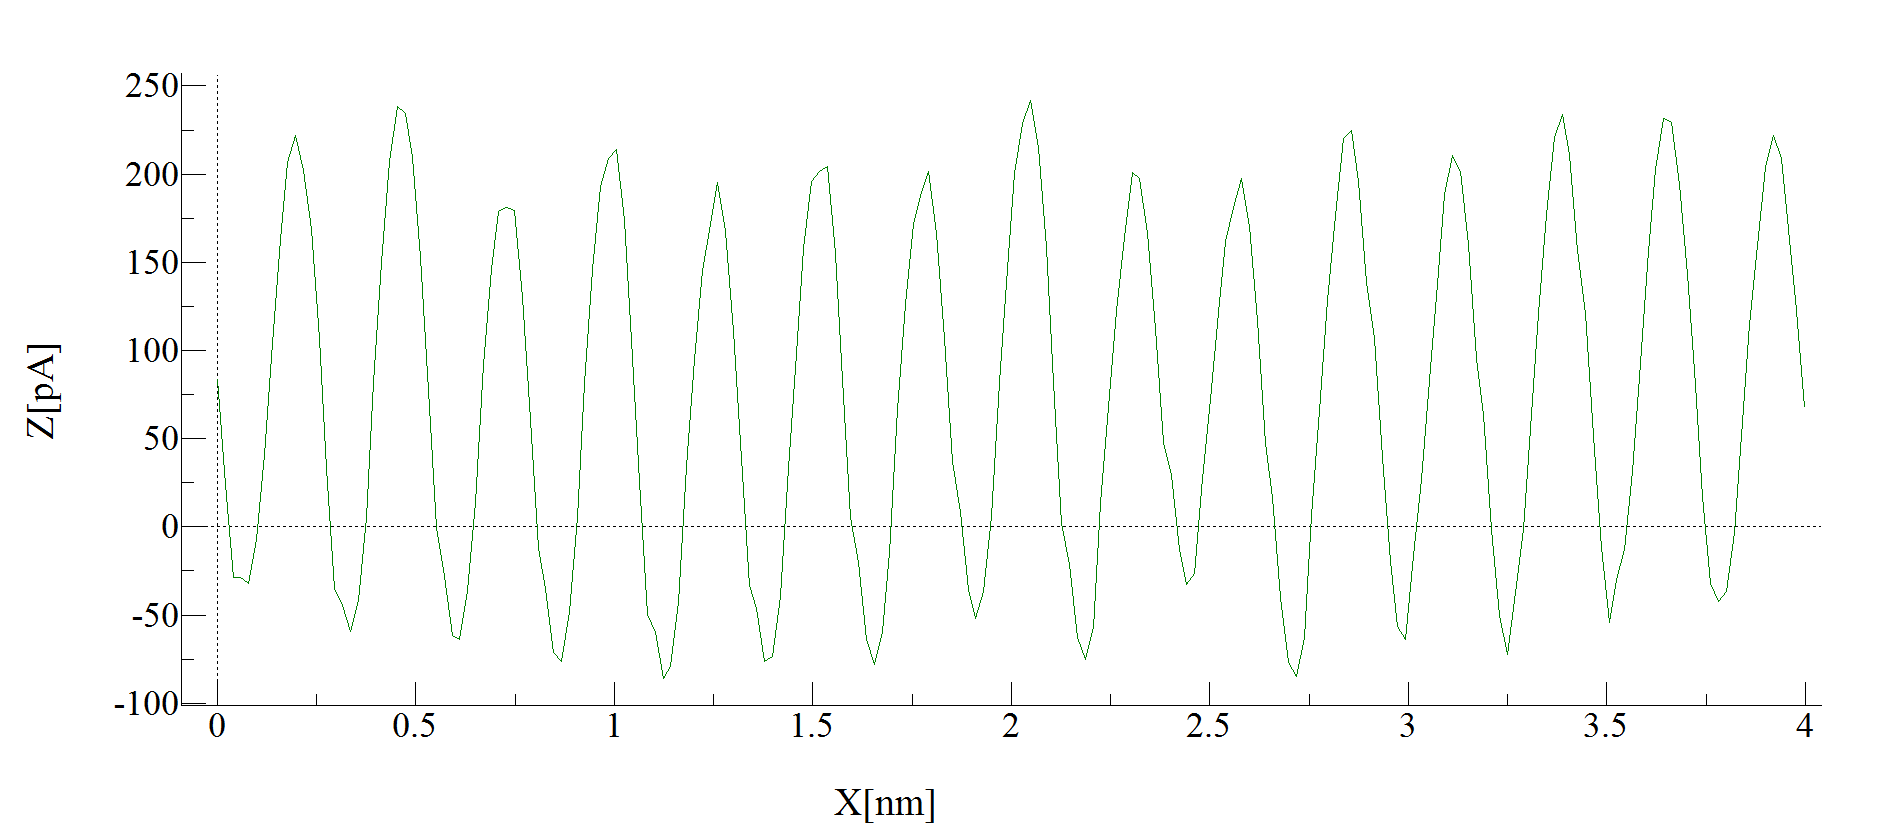
\includegraphics[scale = 0.3]{Aufnahme_Ebene_doppelte_fourier.png}
	
	\caption{Diagramm zur Messung der Abstände der atomaren Erhebungen}
	\label{Messungerh2}
\end{figure}

Zur Messung der Höhe der atomaren Erhebungen mussten wir die Messdaten, die die Höhen und nicht den Tunnelstrom angeben verwenden. Auf diesen Messdaten waren die atomaren Erhebungen selbst nach einer doppelten Fouriertransformation nicht sehr klar zu erkennen, wie in Abbildung \ref{Messungerh3} zu sehen ist. Wir haben entlang der in Abbildung \ref{Messungerh3} zu sehenden Geraden gemessen. Das zu der Geraden gehörende Diagramm kann in \ref{Messungerh4} gesehen werden. An diesem Diagramm haben wir durch das Bilden der Differenz von Maxima und Minima die Höhen der atomaren Erhebungen gemessen. Die Werte können in Tabelle \ref{Messungerh5} gesehen werden. Nach dem Bilden eines Mittelwerts und einer Standardabweichung haben wir für den Wert der Höhe $(8,8 \pm 0,4) pm$.

Der theoretische Wert für den Abstand benachbarter Ebenen in Grafit ist $335 pm$. Dieser Wert übersteigt bei weitem die von uns gemessene Höhe der atomaren Erhebungen. Folglich lassen sich unsere gemessenen Höhen nicht mit diesem Wert identifizieren. Um nachzuvollziehen, wie unsere gemessenen Höhen für die atomaren Erhebungen zustande kommen, müssen wir die Form der Metallspitze, die wir als Sensor benutzen, mit in Betracht ziehen. Diese Spitze hat einen gewisses Ausmaß und kann, wenn es als äußerstes Orbital ein s-Orbital hat, als eine Kugel mit gewissen Radius verstanden werden. Lässt der Tunnelstrom zwischen Sensor und Probe nach, fährt dieser näher an die Probe ran. Dies ist zum Beispiel zwischen den atomaren Erhebungen der Fall. Weil die Metallspitze jedoch einen Radius hat wird es auch, wenn es über einer Stelle zwischen den atomaren Erhebungen ist, mit diesen beim Versuch sich der Probe anzunähern "zusammenstoßen". Deshalb sind die gemessenen Höhen der atomaren Erhebungen viel kleiner als der tatsächliche Ebenenabstand.

\begin{figure}[h]
	\centering
	
	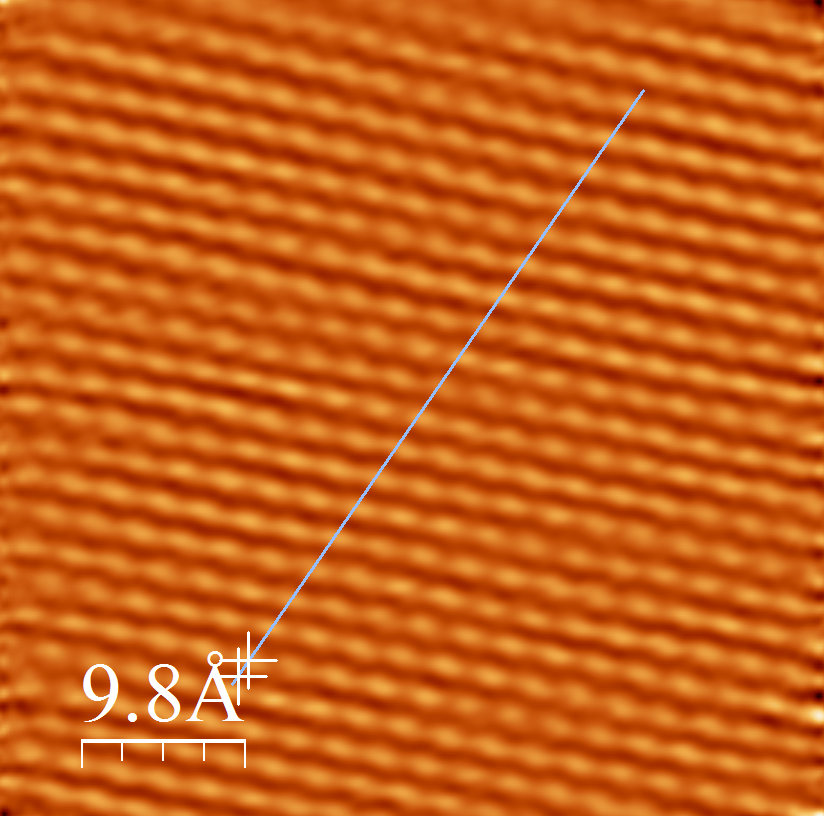
\includegraphics[scale = 0.4]{hohenmessung11.png}
	
	\caption{Messung der Höhe der atomaren Erhebungen}
	\label{Messungerh3}
\end{figure}

\begin{figure}[h]
	\centering
	
	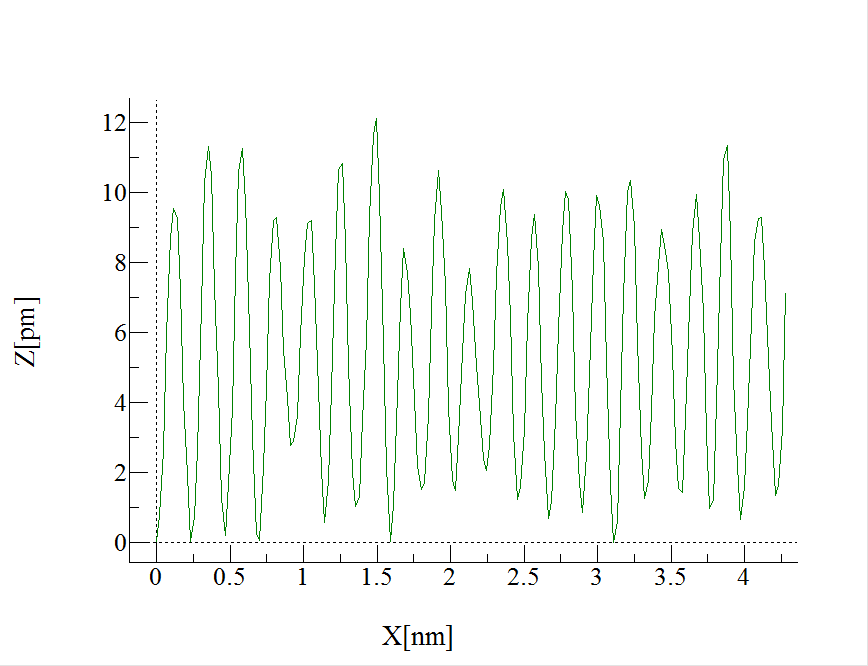
\includegraphics[scale = 0.7]{hohenmessung1_diagramm.png}
	
	\caption{Diagramm zur Messung der Höhe der atomaren Erhebungen}
	\label{Messungerh4}
\end{figure}

\begin{table}[h!]
	\centering
	\begin{tabular}{|l|r|c|lrp{16cm}}\hline
		Abstand/nm & Höhe/pm\\\hline
		0,262 & 9,364 \\
		0,27 & 10,901 \\
		0,264 & 10,967\\
		0,259& 6,444 \\
		0,259 & 8,436 \\
		0,267 & 9,675 \\
		0,264 & 11,881\\
		0,27 & 6,705\\
		0,262 & 9,023\\
		0,27 & 5,687\\
		0,262 & 8,74\\
		0,277 & 8,513\\
		0,262 & 8,829\\
		0,27 & 9,606\\
		& 8,773\\
		& 7,371\\
		& 8,671\\
		& 10,187\\
		& 7,835\\
		\hline
	\end{tabular}
	\caption{Gemessene Werte für die Abstände und Höhen der atomaren Erhebungen}
	\label{Messungerh5}
\end{table}

Anhand von Abbildung \ref{Messungerh6} haben wir die Winkel zwischen den atomaren Richtungen gemessen. Unsere gemessenen Winkel, startend von dem Winkel rechts oben und dann entgegen dem Uhrzeigersinn laufend sind $63^\circ$, $67^\circ$, $48^\circ$, $67^\circ$, $66^\circ$ und $49^\circ$, mit jeweils einem Fehler von $1^\circ$. Wegen der hexagonalen Struktur von Grafit wäre bei einer naiven Herangehensweise zu erwarten, dass alle Winkel $60^\circ$ sind. Dies ist nicht der Fall. Es fällt auf dass die besonders kleinen Winkel($48^\circ$ und $49^\circ$) entgegengesetzt voneinander liegen. Die unterstützt die Theorie, dass die Winkel deshalb alle unterschiedlich groß sind, weil wir nicht senkrecht auf die Grafitprobe gucken.

 Eine andere Erklärung für die unterschiedlichen Winkel könnte daran liegen, dass der Sensor in einem Raster über die Probe fährt. Dabei könnte es zu einem Umrechnungsfehler bei der Berechnung des Bildes aus den Rasterpunkten kommen. Wir halten diese Theorie als weit unwahrscheinlicher, als die, dass wir nicht senkrecht auf die Probe gucken.
 
 Weil von uns beobachteten atomaren Erhebungen der Grafits bilden ein hexagonales Kristallgitter. Es ist 6-zählig. Entlang einer Translation von ganzzahligen Abständen der atomaren Erhebungen der in \ref{Messungerh6} eingezeichneten Linien, gibt es außerdem eine Tanslationssymmetrie. Zusätzlich sieht man, dass bei einer Spiegelung entlang einer der Geraden und einer Inversion an dem Punkt, in dem sich die Geraden schneiden, das Gitter symmetrisch ist.

\begin{figure}[h]
	\centering
	
	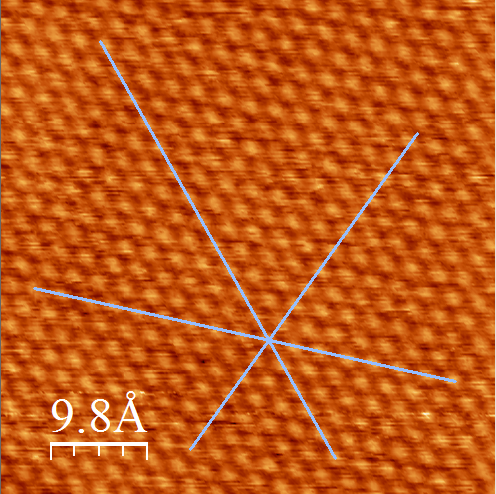
\includegraphics[scale = 0.7]{Winkelmessung_kristall.png}
	
	\caption{Messung der Winkel zwischen den atomaren Richtungen}
	\label{Messungerh6}
\end{figure}

\subsection{Fouriertransformation einer ebenen Fläche Grafits}

In Abbildung \ref{fouriertansformation_ebene} kann das Gitter aus Abbildung \ref{grafob1} nach einer Fouriertransformation betrachtet werden. Man erkennt sechs Punkte, die auf einem leicht verzerrten Hexagon um den Ursprung liegen. Um den Ursprung herum sieht man Werte in geringer Intensität. Dies sind die Störungen, die beim Aufnehmen der Messung entstanden sind. Die sechs zu erkennenden Punkte beinhalten alle Informationen über die Periodizität den gemessenen Gitters. Jedem der sechs Punkte kann ein Vektor $\vec{k}$ zugeordnet werden. Dies ist ein Wellenvektor, der eine Periodizität des Gitter angibt. Verschiebt man das Gitter also um eine Periode der Welle, die mit dem Wellenvektor $\vec{k}$ zu assoziieren ist, bleibt das Gitter unverändert. Daraus lässt sich leicht folgern, dass man aus $\vec{k}$ direkt den Abstand zweier atomarer Erhebungen berechnen kann durch.

\begin{equation}
	|k| = \frac{2\pi}{a}
\end{equation}

Hier ist a der Abstand zweier atomarer Erhebungen

\begin{figure}[h]
	\centering
	
	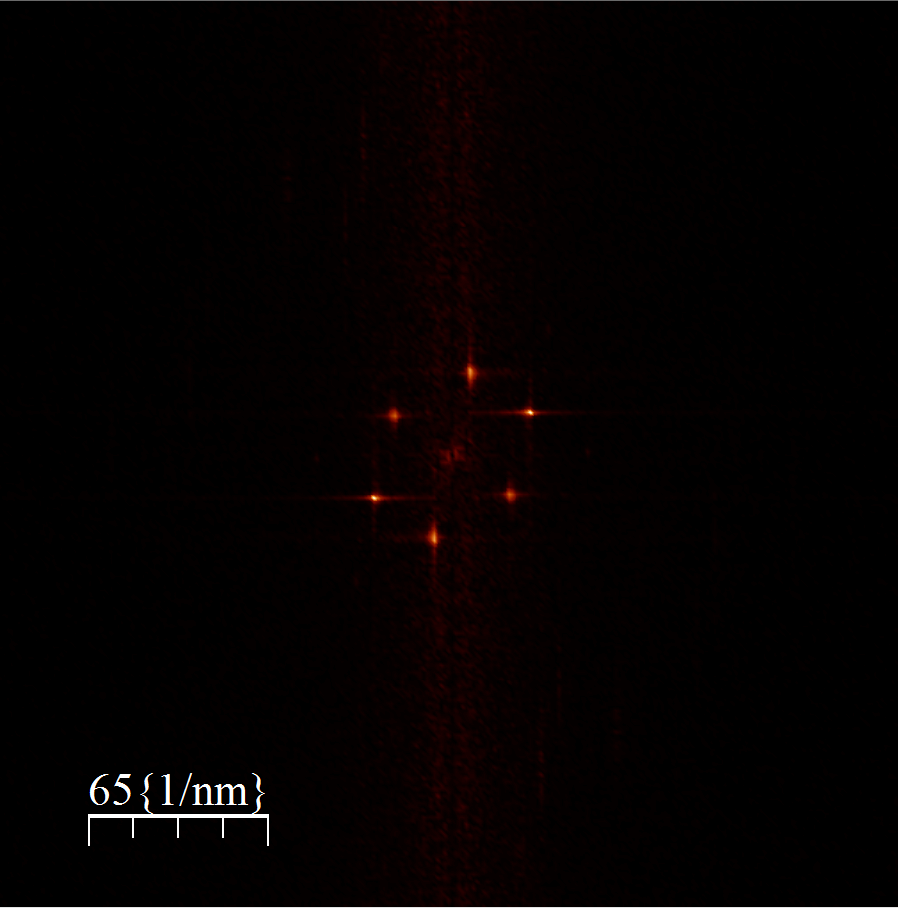
\includegraphics[scale = 0.5]{Fouriertrasformation_kristall.png}
	
	\caption{Fouriertransformation von Abbildung \ref{grafob1}}
	\label{fouriertansformation_ebene}
\end{figure}
\end{document}